\documentclass{article}
\usepackage[UTF8]{ctex}
% Replace `letterpaper' with`a4paper' for UK/EU standard size
\usepackage[a4paper,top=2cm,bottom=2cm,left=3cm,right=3cm,marginparwidth=1.75cm]{geometry}

% Useful packages
\usepackage{amsmath}
\usepackage{graphicx}
\usepackage[colorlinks=true, allcolors=blue]{hyperref}
\usepackage{graphicx} %插入图片的宏包
\usepackage{float} %设置图片浮动位置的宏包
\usepackage{subfigure} %插入多图时用子图显示的宏包
\usepackage{parskip}
\usepackage{indentfirst} 
\setlength{\parindent}{2em}
\usepackage{hyperref}  
\usepackage{tikz}
\allowdisplaybreaks
\usepackage{multirow}
\usepackage{amsmath}
\usepackage{amsfonts,amssymb} 
\usepackage{xcolor} % 用于显示颜色
\usepackage{listings} % 用于插入代码
\lstset{
	basicstyle          =   \sffamily,          % 基本代码风格
	keywordstyle        =   \bfseries,          % 关键字风格
	commentstyle        =   \rmfamily\itshape,  % 注释的风格,斜体
	stringstyle         =   \ttfamily,  % 字符串风格
	flexiblecolumns,                % 别问为什么,加上这个
	numbers             =   left,   % 行号的位置在左边
	showspaces          =   false,  % 是否显示空格,显示了有点乱,所以不现实了
	numberstyle         =   \zihao{-5}\ttfamily,    % 行号的样式,小五号,tt等宽字体
	showstringspaces    =   false,
	captionpos          =   t,      % 这段代码的名字所呈现的位置,t指的是top上面
	frame               =   lrtb,   % 显示边框
}

\lstdefinestyle{Python}{
	language        =   Python, % 语言选Python
	basicstyle      =   \zihao{-5}\ttfamily,
	numberstyle     =   \zihao{-5}\ttfamily,
	keywordstyle    =   \color{blue},
	keywordstyle    =   [2] \color{teal},
	stringstyle     =   \color{magenta},
	commentstyle    =   \color{red}\ttfamily,
	breaklines      =   true,   % 自动换行,建议不要写太长的行
	columns         =   fixed,  % 如果不加这一句,字间距就不固定,很丑,必须加
	basewidth       =   0.5em,
}

\title{数据结构第二次上机实验报告}
\author{林子开}

\begin{document}
	\maketitle
	\tableofcontents

\section{Ordinary algorithm的时间复杂度}
\subsection{理论分析}
Ordinary算法的核心部分如下:

\lstinputlisting[style = Python,
caption={ordinary algorithm核心部分},
label = {ord1},
linerange={7-15}]{ordinary_algorithm_for_matrix_multiplication.py} 

\par 为便于讨论,只考虑矩阵$A$和矩阵$B$均为维度大小为$n$的方阵的情况。$C=AB$,在计算$C$中的每个元素$C_{ij}$时,需要计算$n$次乘法和$n$次加法,复杂度为$\Theta(n)$,由于$C$中一共有$n^2$个元素,则Ordinary algorithm算法的时间复杂度为$\Theta(n^3)$。

\subsection{实验结果}
分别对矩阵大小$n=2^3,2^4,2^5,2^6,2^7,2^8$的情况进行测试,实验结果如表\ref{ord-result}所示
\begin{table}[H]
	\centering
	\caption{Ordinary Algorithm的实验结果}
	\label{ord-result}
	\begin{tabular}{lllllll}
		\hline
		矩阵维度$n$         & $2^3$ & $2^4$ & $2^5$ & $2^6$ & $2^7$ & $2^8$ \\ \hline
		time/s     & 0.000167             & 0.002                & 0.016504             & 0.126088             & 1.028406             & 7.999888             \\
		$\log_2(\text{time})$ & -12.5502             & -8.96548             & -5.92106             & -2.98749             & 0.04041              & 2.99998              \\ 
		\hline
	\end{tabular}
\end{table}

\par 做出“运行时间-矩阵大小”的双对数图如下
	\begin{figure}[H]
			\centering  %图片全局居中
			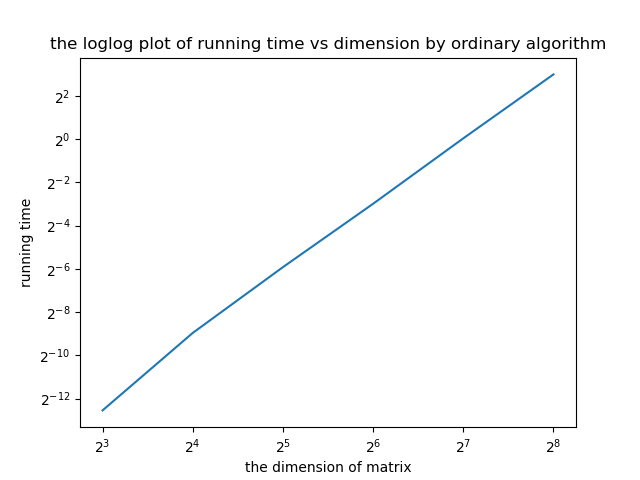
\includegraphics[width=0.8\textwidth]{ord}
			\caption{ordianry algorithm的时间复杂度双对数}
		\end{figure}

\par 并对$\log_2(\text{time})$与$\log_2(n)$用R语言做线性回归(即最小二乘法),得到拟合直线的斜率,得到斜率$k=3.077$。

\subsection{小结} 可以看出,实验结果与理论分析较为一致,ordinary algorithm算法的时间复杂度确实为$\Theta(n^3)$。



\section{Strassen's algorithm的时间复杂度}
\subsection{理论分析}
为便于讨论,在这一部分,对于$C=AB$,仍假设$A,B$均为方阵,大小为2的整数幂次,以便进行矩阵分块。

Strassen's algorithm分为以下几个步骤:
\begin{enumerate}
	\item 递归基础情况,时间复杂度$\Theta(1)$
		\lstinputlisting[style = Python,
		caption={Strassen's algorithm递归基础情况},
		label = {st1},
		linerange={5-10}]{Strassen_algorithm_for_matrix_multiplication.py} 
	
	\item 矩阵分块,时间复杂度$\Theta(1)$
		\lstinputlisting[style = Python,
		caption={Strassen's algorithm矩阵分块},
		label = {st3},
		linerange={13-21}]{Strassen_algorithm_for_matrix_multiplication.py}
	
	\item 做10个矩阵加减法,生成$S_1\sim S_{10}$,时间复杂度$\Theta(n^2)$
		\lstinputlisting[style = Python,
		caption={Strassen's algorithm 矩阵加减法生成辅助矩阵S1到S10},
		label = {st4},
		linerange={24-33}]{Strassen_algorithm_for_matrix_multiplication.py}
	
	\item 做7个矩阵乘法,使用递归方法,生成$P_1\sim P_7$,时间复杂度\textbf{$7T(\frac{n}{2})$}
		\lstinputlisting[style = Python,
		caption={Strassen's algorithm 使用递归方式计算矩阵乘法,生成辅助矩阵P1到P7},
		label = {st5},
		linerange={36-42}]{Strassen_algorithm_for_matrix_multiplication.py}

	\item 做8个矩阵加减法,生成分块矩阵$C_1\sim C_4$,时间复杂度$\Theta(n^2)$
		\lstinputlisting[style = Python,
		caption={Strassen's algorithm 矩阵加减法生成分块矩阵C1到C4},
		label = {st6},
		linerange={45-48}]{Strassen_algorithm_for_matrix_multiplication.py}

	\item 分块矩阵拼接,时间复杂度$\Theta(1)$
		\lstinputlisting[style = Python,
		caption={Strassen's algorithm 矩阵拼接},
		label = {s7},
		linerange={50-52}]{Strassen_algorithm_for_matrix_multiplication.py}
\end{enumerate}
	\par 由上述讨论可知,Strassen's algorithm的时间复杂度满足递推公式
	\[ T(n) = 7T(\frac{n}{2}) + \Theta(n^2) \]
	由于$n^2 = O(n^{log_2 7 - \epsilon}),\, \epsilon = log_27 - 2 \approx 0.807 > 0$,
	根据Master Method可知,
	\[T(n) = \Theta(n^{\log_2 7}) \approx \Theta(n^{2.80735})\]


\subsection{实验结果}
	分别对矩阵大小$n=2^3,2^4,2^5,2^6,2^7,2^8$的情况进行测试,实验结果如表\ref{st-result}所示
	\begin{table}[H]
	\centering
	\caption{Strassen's Algorithm的实验结果}
	\label{st-result}
	\begin{tabular}{lllllll}
	\hline
	矩阵维度$n$         & $2^3$ & $2^4$ & $2^5$ & $2^6$ & $2^7$ & $2^8$ \\ 
	\hline
	time/s      & 0.00183384           & 0.01380310           & 0.09567207           & 0.65380581           & 4.57863772           & 31.94628000          \\
	$\log_2(\text{time})$ & -9.09091947          & -6.17886381          & -3.38575836          & -0.61306589          & 2.19491842           & 4.99757604           \\ 
	\hline
	\end{tabular}
	\end{table}

\par 做出“运行时间-矩阵大小”的双对数图如下
	\begin{figure}[H]
			\centering  %图片全局居中
			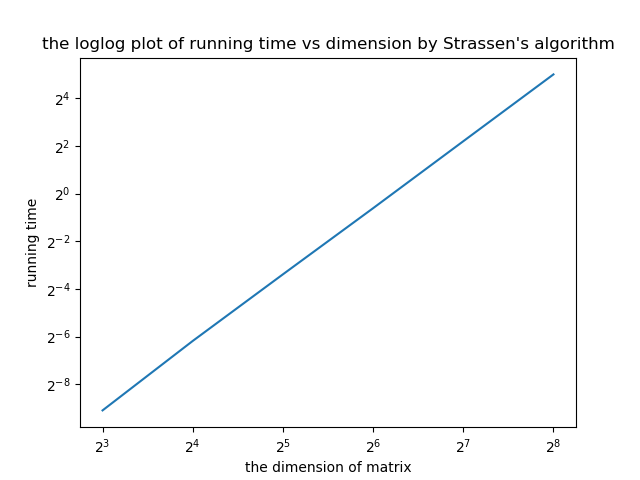
\includegraphics[width=0.8\textwidth]{Strassen}
			\caption{Strassen's algorithm的时间复杂度双对数}
		\end{figure}

\par 并对$\log_2(\text{time})$与$\log_2(n)$用R语言做线性回归(即最小二乘法),
得到拟合直线的斜率,得到斜率$k=2.80962$。


\subsection{小结} 可以看出,实验结果与理论分析较为一致,
Strassen's algorithm算法的时间复杂度确实为$\Theta(n^{\log_2 7})$。

\section{附录A:ordinary algorithm完整源代码}
\lstinputlisting[style = Python,
caption={ordinary algorithm 完整python源码},
label = {ord-complete}]{ordinary_algorithm_for_matrix_multiplication.py} 


\section{附录B:Strassen's algorithm完整源代码}
\lstinputlisting[style = Python,
caption={Strassen's algorithm 完整python源码},
label = {st-complete}
]{Strassen_algorithm_for_matrix_multiplication.py}

\end{document}